\documentclass{report}

\usepackage[utf8]{inputenc}
\usepackage[T1]{fontenc}
\usepackage[french]{babel}

\usepackage{lmodern}

\usepackage{setspace}
\spacing{1.5}

% \makeatletter
% \@addtoreset{chapter}{part}
% \makeatother  

\usepackage{url}

\usepackage{graphicx}

\newcommand{\emphbox}[1]{
    \noindent\fbox{
        \begin{minipage}[c]{\linewidth}
            {\em #1}
        \end{minipage}
    }
}

\title{Extraction de données relatives aux produits alimentaires à partir de documents non structurés}
\author{Pierre \textsc{massé}}
\date{Juin 2020}

\begin{document}

\maketitle

\large
\begin{abstract}
    {\em
    
    La gestion de l'information produit est devenu un enjeu de société majeur ces dernières années.
    Les scandales sanitaires récents ont déclenché une prise de conscience collective des consommateurs, en parallèle de la mise en place de réglementations de plus en plus contraignantes pour l'ensemble des acteurs de la filière\cite{incotext}\cite{incoexpl}.
    \`{A} ce titre, le Groupe Pomona a lancé ces dernières années un projet majeur de refonte des processus et des outils de gestion de l'information produit.

    La première filiale du Groupe a fait l'objet d'un déploiement réussi, mais cela a toutefois mis en évidence le fait que des gains à la fois en qualité et en productivité restent accessibles.

    La mise en place d'outils mettant en oeuvre les principes du Machine Learning appliqués au traitement du langage permettrait d'aider les opérationnels de la gestion de l'information à interpréter plus vite et mieux les documents mis à disposition par les fournisseurs du Groupe.

    Le présent rapport détaille la mise en place d'un outil permettant d'extraire les listes d'ingrédients des fiches techniques transmises par les fabricants des produits.
    }
\end{abstract}
\normalsize

\tableofcontents

\part{Contexte métier}

    \chapter{Description du Groupe}

    \large
    L'objet de l'ensemble de cette première partie est de donner sur le Groupe Pomona des éclairages nécessaires à la compréhension du cas d'usage développé.
    Bien d'autres aspects sur la société, pourraient être mentionnés (ex : des indicateurs sur l'activité, l'histoire du Groupe\dots) mais ils seront omis car non indispensables à la compréhension du sujet.
    Plus de détails sur le Groupe sont accessibles sur le site web de la société\cite{site_pomona}.
    \normalsize    

        \section{Le métier du Groupe Pomona}

        Le Groupe Pomona est une société de distribution livrée de produits alimentaires à destination des professionnels des métiers de bouche.
        L'activité du Groupe consiste uniquement à acheter et revendre de la marchandise, à l'exclusion de toute activité de fabrication ou de transformation\footnote{de très rares cas de transformation existent (ex : mûrissage de fruits, filetage de poisson) mais extrêmement exceptionnels}. Le Groupe Pomona est une société de \emph{distribution}. Elle ne possède d'ailleurs pas d'actif industriels (autre que des entrepôts logistiques) ni d'agréement 
        
        
        Cette activité d'achat/vente se fait dans la majorité des cas sous le régime du \emph{négoce}, à savoir que le Groupe acquiert la propriété des marchandises qu'il commercialise avant de la céder à ses clients.
        L'autre régime est celui dit de la \emph{prestation (logistique)}.
        Dans ce cas, par le jeux d'écritures comptables, la valorisation du stock disparaît des comptes du Groupe.
        Néanmoins, indépendamment de cet aspect purement comptable, l'ensemble :
        \begin{description}
            \item[des flux de documents :] commandes d'achat, factures fournisseur, commandes de vente, factures clients
            \item[des flux financiers :] paiements fournisseur, paiements client
            \item[des flux physiques :] réception et stockage, préparation et expédition
        \end{description}
        restent largement inchangés.
        
        Pour résumer, l'activité de l'ensemble des entités du Groupe pourraient se résumer via le schéma présenté en figure \ref{fig:flux metier}

        \begin{figure}[htbp]
            \begin{center}
            \includegraphics[width=\linewidth]{img/Les flux métier de Pomona.png}
            \end{center}
            \caption{Les flux métier avec les partenaires commerciaux}
            \label{fig:flux metier}
        \end{figure}

        \emphbox{Le métier du Groupe est d'être un \emph{grossiste}, qui achète et revend des produits alimentaires\footnotemark \ \emph{sans produire ou transformer quoi que ce soit}.}
        \footnotetext{dans la grande majorité des cas, cf. paragraphes suivants}

        \section{La décentralisation}
        
        Le Groupe Pomona est un Groupe fortement décentralisé, avec des organisations largement indépendantes les unes des autres. 

            \subsection{Les Directions fonctionnelles}

            Pour des raisons évidentes de recherche de synergies ou de conformité réglementaires, certaines activités restent toutefois mutualisées à la maille du Groupe.
            Il s'agit des organisations suivantes :
            \begin{description}
                \item[La Direction Administrative et Financière (DAF) :] regroupe les équipes comptables Groupe, l'audit interne et la consolidation financière
                \item[La Direction Qualité :] est en charge de définir et contrôler l'application des standard de qualité
                \item[La Direction des Systèmes d'Information (DSI) :] développe et maintient en condition opérationnelles les systèmes d'information du Groupe
                \item[La Direction Technique et Logistique (DTL) :] est en charge des projets immobiliers (entrepôts), des négociations avec les transporteurs et joue un rôle de conseil interne sur les sujets logistiques
                \item[La Direction des Ressources Humaines :] se charge de l'ensemble des aspects en lien avec le recrutement, la paye et les sujets sociaux
                \item[La Direction Commerciale Groupe (DCG) :] définit une stratégie et des bonnes pratiques commerciales et marketing
            \end{description}

            \subsection{Les clients du Groupe}
            \label{clients}

            Afin de comprendre l'organisation du Groupe, il est nécessaire de connaître la typologie de ses clients.
            Comme mentionné précédemment, le Groupe s'adresse exclusivement aux professionnels des métiers de bouche.
            Aucune marchandise n'est vendue à des particuliers.
            Les principales typologies de clients sont les suivantes : 
            \begin{description}
                \item[Les Sociétés de Restauration :] elles exploitent les restaurants d'entreprise et certaines cantines d'établissement d'enseignement supérieur
                \item[Les Marchés Publics :] regroupent les clients qui dépendent des collectivités (écoles, hôpitaux, prisons, \dots)
                \item[La restauration commerciale :] est l'ensemble des restaurants à vocation commerciale, qu'ils soient chaînés (hippopotamus, O'Tacos, \dots) ou indépendants (\og le restaurant du coin \fg)
                \item[Les spécialistes :] il s'agit des détaillants spécialisés qui s'adressent aux particuliers. Boulangers, pâtissiers, bouchers, traiteurs, vente à emporter, \dots
                \item[Les Grandes et Moyennes surfaces (la GMS) :] sont les enseignes de la grande distribution. En général, l'accès à ces clients est compliqué par les règles mises en place par leurs centrales d'achat. Il représentent en général qu'un canal de vente d'opportunité.
            \end{description}

            Les trois premières de ces catégories représentent ce que l'on appelle la \emph{Restauration Hors Domicile (RHD)} (ou parfois également la Restauration Hors Foyer, RHF).

            \subsection{Premier niveau de décentralisation : les branches}
            
            Le Groupe Pomona est divisé en branches, qui sont des organisations indépendantes et qui ont toute latitude pour gérer leurs stratégie et politique commerciales, la gestion de leurs achats, leur stratégie marketing, \dots
            Afin d'éviter de se concurrencer entre elles, leurs domaines d'activité respectifs ont été partitionnés par familles de produit commercialisés, segments client cibles et géographie. 

                \subsubsection{Les branches RHD}
                
                Les branches RHD s'adressent comme leur nom l'indique aux client de la Restauration Hors Domicile (cf. section \ref{clients} page \pageref{clients}) en France.
                Elles se répartissent ce marché en travaillant des gammes de produits distinctes.
                Il s'agit des branches historiques du Groupe, qui représentent l'essentiel de son chiffre d'affaire.
                La répartition par produit est la suivante :
                \begin{description}
                    \item[PassionFroid :] spécialiste des \emph{produits surgelés, de la viande fraîche et des produits laitiers}
                    \item[\'{E}piSaveurs :] spécialiste des produits qui se conservent à température ambiante : \emph{produits d'épicerie, conserves, boissons et consommables de cuisine non-alimentaires}
                    \item[TerreAzur :] spécialites des \emph{Fruits et Légumes frais, et Produits De la Mer frais} 
                \end{description}
                La non-concurrence entre les branches est assurée par le fait qu'elles ne commercialisent pas les mêmes produits.
                Bien que nommées RHD, elles peuvent également vendre leurs produits à la grande distribution, mais généralement ces marchés sont verrouillés par les centrales d'achat des grandes enseignes.

                \subsubsection{Les branches spécialistes}

                Les branches spécialistes s'adressent aux clients dits spécialistes (cf. section \ref{clients} page \pageref{clients}) en France.
                Elles sont en mesure de commercialiser tout type de produit pour répondre aux besoins de leurs clients.
                En particulier, elles peuvent tout à fait commercialiser certains produits qui sont également vendus par les branches RHD.
                Elles se répartissent la clientèle spécialiste de la manière suivante :
                \begin{description}
                    \item[Délice et Création :] s'addresse aux \emph{Boulangers et Pâtissiers}
                    \item[Saveurs d'Antoine :] s'adresse aux \emph{Bouchers, Charcutiers et Traiteurs}
                    \item[Relais d'Or :] s'addresse à la \emph{restauration indépendante nomade}
                \end{description}
                Comme pour les branches RHD, ces branches peuvent lorsqu'elles en ont l'opportunité vendre leurs produits à la GMS.

                \subsubsection{L'étranger}

                Bien que le Groupe Pomona soit une société dont l'essentiel de l'activité est faite sur le marché français, deux réseaux sont en cours de constitution sur des pays limitrophe.
                Ces branches sont susceptibles de travailler tout type de produit, à destination de tout type de client.
                Elles sont positionnées sur les marchés suivants : 
                \begin{description}
                    \item[Pomona Suisse :] présente sur le marché Suisse
                    \item[Pomona Iberia :] présente sur le marché Espagnol 
                \end{description}

                On peut synthétiser la répartition de l'activité par branche de la manière présentée à la figure \ref{fig:repartition_activite}.
                \begin{figure}[htpb]
                    \begin{center}
                    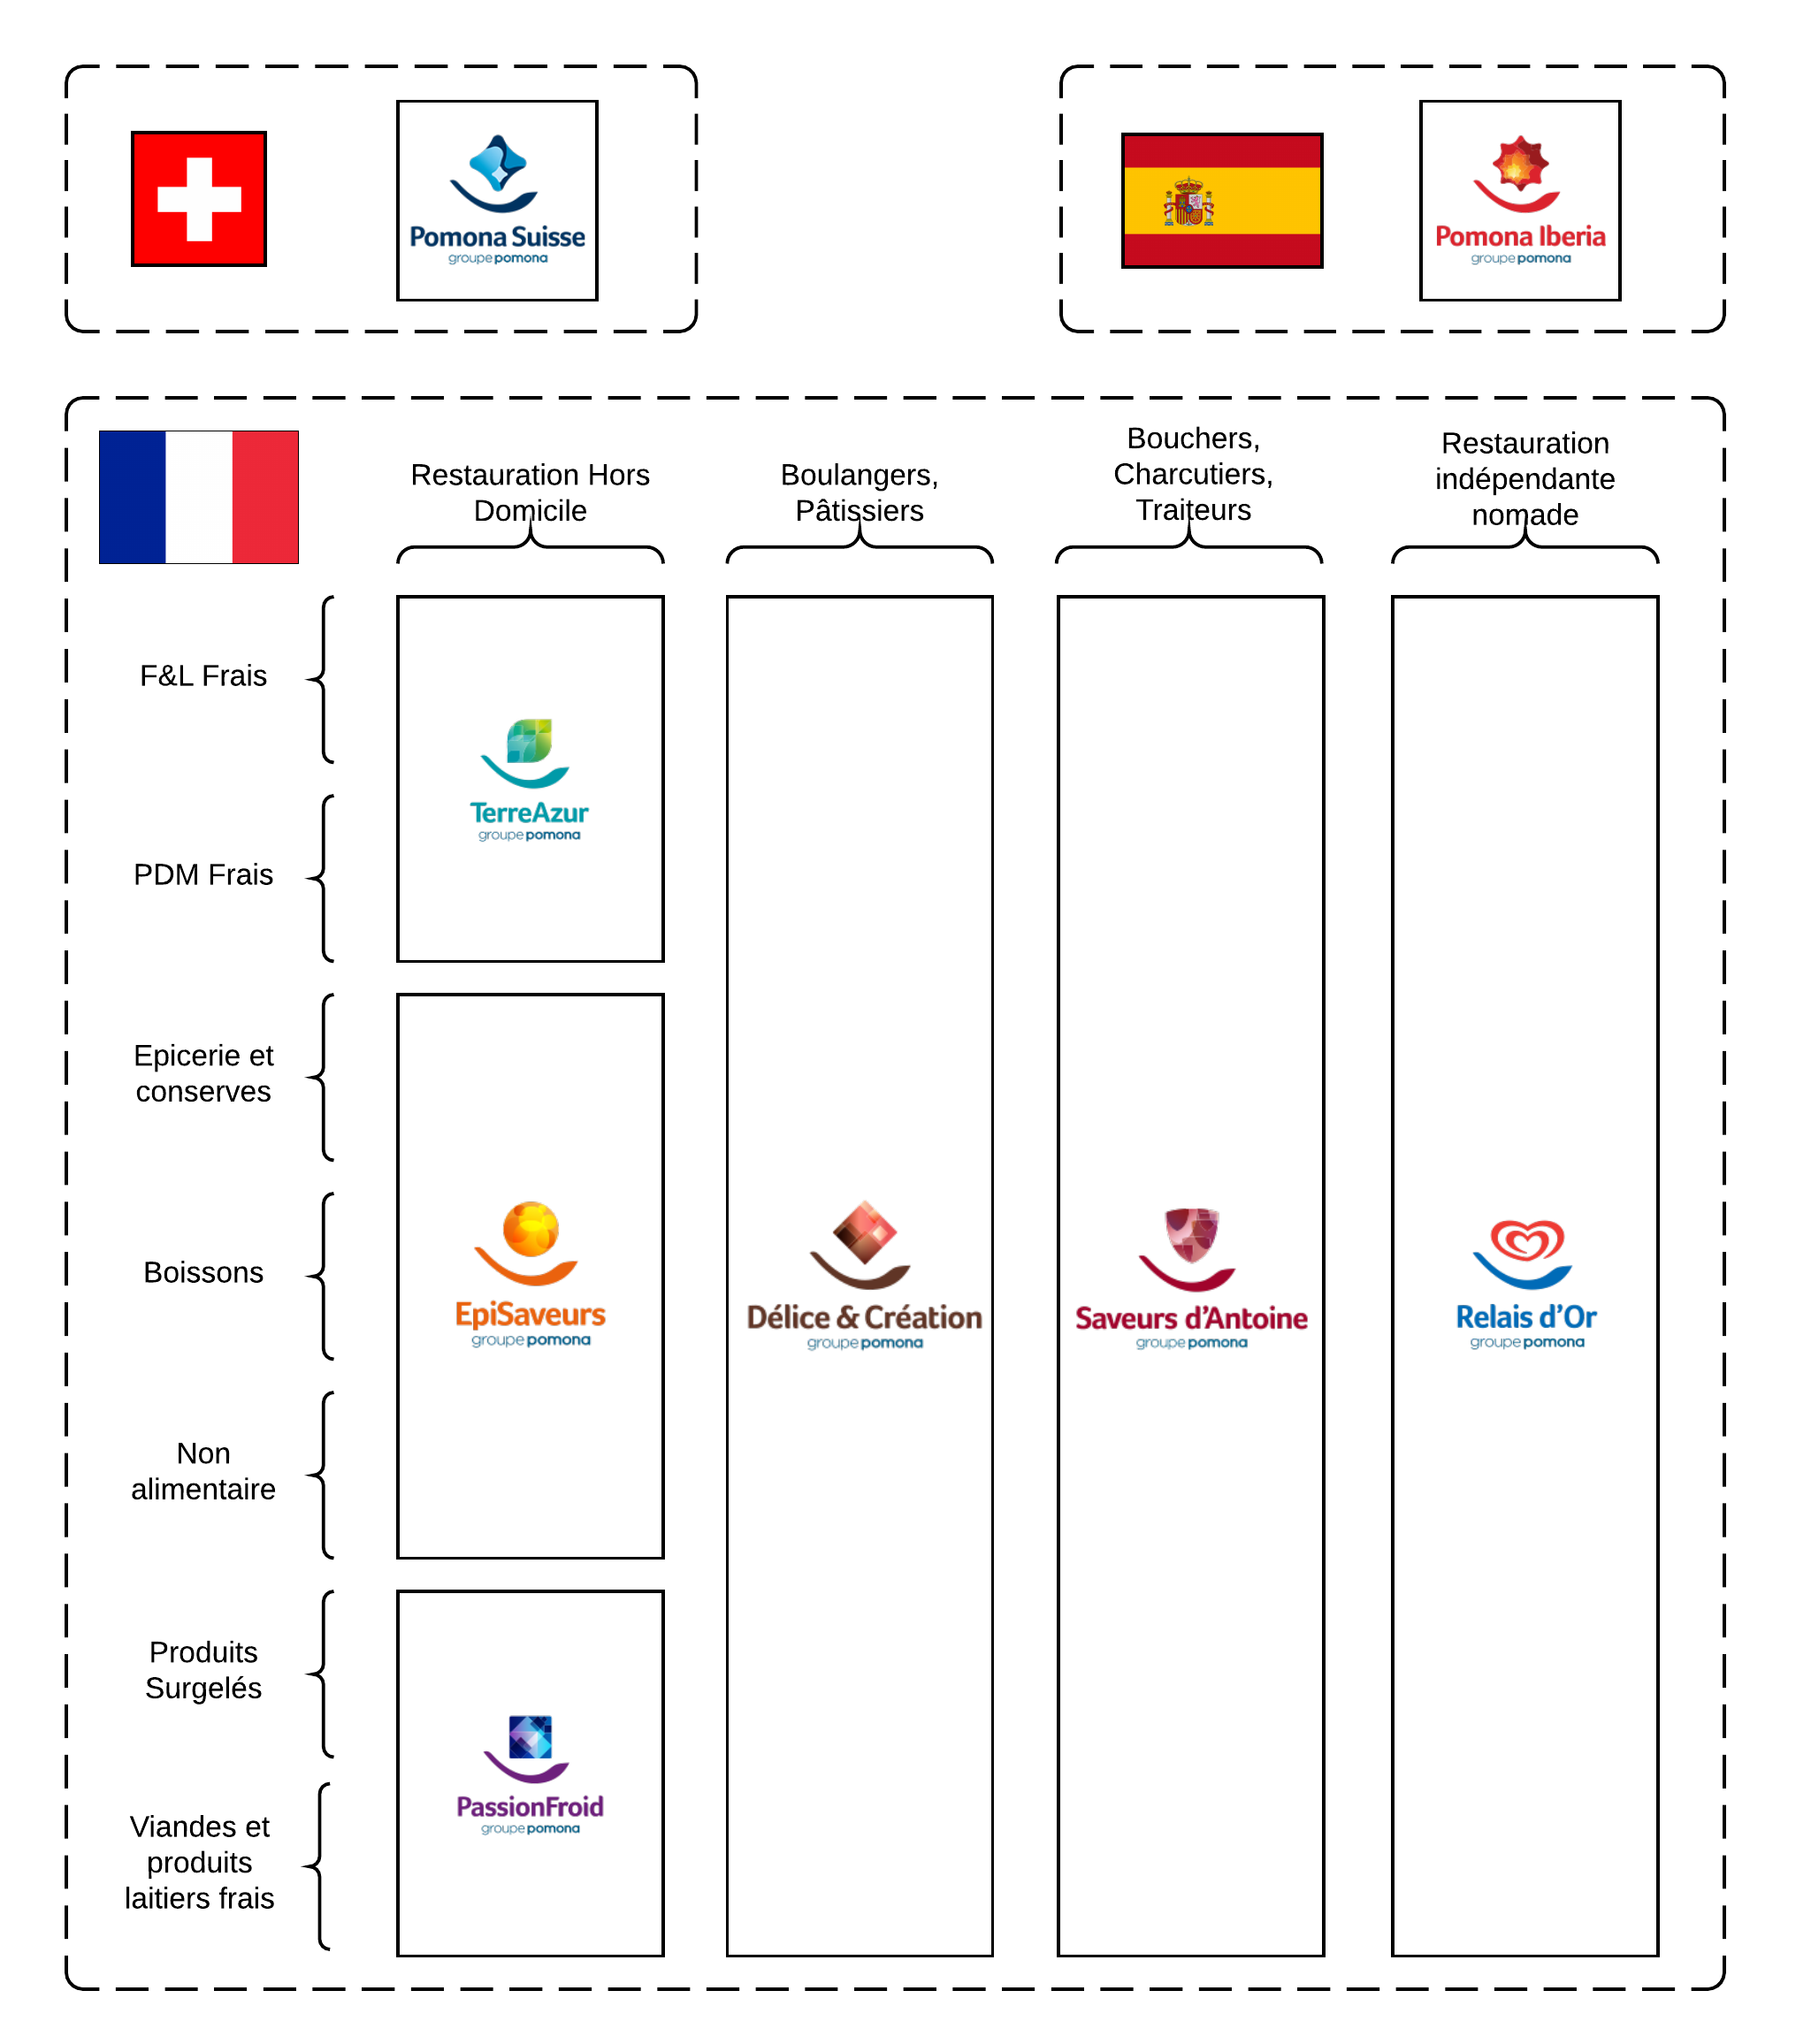
\includegraphics[width=\linewidth]{img/La répartition de l'activité des branches.png}
                    \end{center}
                    \caption{La répartition de l'activité des branches}
                    \label{fig:repartition_activite}
                \end{figure}

            \subsection{Le second niveau de décentralisation : les succursales}

            Chacune des branches est elle-même à son tour décentralisée en un réseau d'entrepôts régionaux : les succursales (parfois également appelées simplement \og régions\fg).
            Ces succursales sont gérées comme des PME indépendantes, avec un directeur et un compte de résultat qui leur est propre.
            Si certaines négociation avec des fournisseurs ou des clients nationaux sont parfois menée par les branches, les succursales sont autonomes dans :
            \begin{itemize}
                \item{la définition de leur assortiment, même si des contraintes s'appliquent}
                \item{la stratégie de développement commercial}
                \item{la négociation des prix d'achat}
                \item{la négociation des prix de vente}
                \item{la politique de rémunération de leurs employés}
            \end{itemize}
            
            \'{A} ce titre, elles ont leurs propres équipes d'achat, leurs équipes commerciales (télévente et vente route), leurs équipes administratives et évidemment leurs équipes logistiques (essentiellement en entrepôt et les chauffeurs livreurs en charge des livraisons client).
            Un exemple de maillage régional est présenté en figure \ref{fig:reseau_es}, sachant que ce maillage régional est différent pour chacune des branches.
            \begin{figure}[htpb]
                \begin{center}
                \includegraphics[width=\linewidth]{img/réseau es.png}
                \end{center}
                \caption{Le maillage régional de la branche \'{E}piSaveurs}
                \label{fig:reseau_es}
            \end{figure}


    \chapter{La gestion de l'information produit}
        \section{L'information produit}
        \section{Le processus associé}
        \section{Le PIM (Product Information Management)}

\part{Les données}
    \chapter{Le périmètre produit}
        \section{Accessibilité de la donnée en fonction des branches}
        \section{Les branches déployées}
        \section{Les types de produit}
    \chapter{Les données utilisables}
        \section{Données structurées}
        \section{Données non structurées}
        \section{Pièces jointes}

            Dans chacune des sections, mentionner la volumétrie de données accessibles (avec les facettes migration, statuts, \& compagnie)

            \subsection{Fiches techniques fournisseur}
            \subsection{\'{E}tiquettes produit}
            \subsection{Fiches logistiques fournisseur}
            \subsection{Fiches techniques et argumentaires Pomona}
        \section{Récapitulatif de la complétude des données}

        Mettre ici un ou plusieurs tableaux récapitulatifs illustrant les données possédées quantitativement.

        \section{Analyse qualitative des données}
        
        Montrer qu'un sondage basique fait que la qualité actuelle est perfectible

        Mettre également la distribution numérique des produits par fournisseur et insister sur la difficulté posée par de multiples formats

        Dire ici qu'il y a finalement beaucoup de pdf qui possèdent des textes extractibles vs. uniquement des images.

        \section{Les données \og manuellement étiquetées \fg}

        Montrer comment elles ont été produites

        Expliciter les règles de gestion qui ont été listées pendant l'étiquetage manuel

        Evaluer la cohérence entre étiquettes manuelles et contenu du PIM

\part{Les objectifs de ce projet}
    \chapter{Les cas d'usage}
        \section{Objectifs : Qualité et productivité}
        \section{La préalimentation d'information}
        \section{Le contrôle à la saisie fournisseur}
        \section{L'aide aux vérifications Pomona}
        \section{Les contrôles en masse asynchrones}
    \chapter{Les types de données à récupérer}
        \section{La composition produit}
        \section{Les données nutritionnelles}
        \section{Les données logistiques}
    \chapter{Le choix du cas d'usage}
        \section{Les multiples formats}
        \section{Les informations \og spatialisées \fg}
        \section{La complexité dans la réprésentation des données logistiques}
        \section{La moindre représentation des étiquettes}
        blablabla
        \newline
        \newline
        \emphbox{Au vu des différentes contraintes listées plus haut, on s'attachera à extraire \emph{les listes d'ingrédients} depuis \emph{les fiches techniques fournisseur}, en se basant sur \emph{le contenu textuel} de ces documents.}

\part{Construction du modèle}
    \chapter{Les principes généraux}
        \section{Contenu du texte d'une liste d'ingrédients}

        Les listes d'ingrédients juste une liste ordonnées d'ingrédients triés par ordre décroissant de quantité mise en oeuvre.

        Parfois détaillé par phase, mais en général déconseillé.

        En général, chaque ingrédient sera présent une seule fois dans la liste.

        Le calcul d'embeddings via des modèles tels que SVD ou Word2Vec fait peu de sens.
        \newline
        \newline
        \emphbox{l'extraction des textes se fait au format \emph{Bag Of Words}, sans utiliser de notion d'IDF. L'utilsation de TF semble églament sujette à caution.}

        \section{Limitation à l'identification des listes d'ingrédients}

        On est sur une taxonomie d'informations limitée dans les fiches techniques.

        On pourrait envisager de classifier l'ensemble des textes présents dans les fiches techniques.

        Mais l'absence de données étiquetées rend cette tâche impossible. La charge d'étiquetage d'un nombre représentatif de blocs de texte de fiches techniques est trop importante pour être mise en oeuvre dans le cadre de ce projet.

        \section{Conversion de documents en texte}
        
        dire ici qu'on utilise principalement pdfminer vs. d'autres outils d'OCR.

        De plus, on partira dans un premier temps sur une transformation basique d'un document en texte, sans passer par une analyse de la localisation des textes sur le document.
            
    \chapter{Construction d'un modèle simple \og ouvert \fg}
        
    Expliciter le principe de ce modèle avec un schéma simple.

    Pas de mesure possible de la performance

        \section{Extraction des données}

        Ne garder que produits d'épicerie et boissons non alcoolisées

        \section{Conversion en blocs de texte}
        \section{Train/Test split}
        \section{Entrainement du modèle}
        \section{Calcul de la similarité}
        \section{Illustration des résultats obtenus}
    
    \chapter{Utilisation des données manuellement étiquetées}

    Expliciter pourquoi on ne peut pas faire tourner (référence parties précédentes) sur l'ensemble des données
        
        \section{Chargement des données manuellement étiquetées}

        \section{Train/Test split}

        \section{Entraînement du modèle}

        \section{Illustration des prédictions obtenues}


    \chapter{Mesure de la performance}
    
        \section{Calcul de la précision}
            \subsection{Approche naïve}

            \subsection{Avec du \og text-postprocessing \fg}
        \section{Calcul d'une \emph{loss}}

        Expliciter les diverses distances, et pourquoi certaines sont plus pertinentes que d'autres.

        Ex : on ne garde pas la distance de Hamming
            \subsection{Distance de Levenshtein}

            \subsection{Distance de Dameray-Levenshtein}

            \subsection{Distance de Jaro}

            \subsection{Distance de Jaro-Wrinkler}
    
        \section{Cross-validation des modèles précédents}
            
            \subsection{Modèle \og ouvert \fg}

            \subsection{Modèle entraîné sur les données étiquetées manuellement}

    \chapter{Transfer learning}
        
        \section{Principe du pré-entraînement}
        
        Expliquer qu'il s'agit d'une approche hybride des 2 modèles précédents

        \section{Illustration de l'impact sur la performance}


    \chapter{Hyperparameter tuning}
            
        \section{Les paramètres ajustables}

        \section{Application d'une grid search}

\part{Travaux subséquents}
    \chapter{Opérationnalisation de cette maquette}    
        \section{Client et sponsor métier}
        \section{Définition des règles de gestion}
        \section{Mise en place d'une organisation projet}
        \section{Industrialisation du code}
        Prochaines étapes : opérationnalisation via API \\
        Documentation
        \section{Monitoring de la performance du modèle}
    \chapter{Extension des fonctionnalités offertes}
        \section{Prise en compte de nouveaux types de pièces jointes}
        \section{Utilisation d'outil d'OCR pour les pdf non structurés}
        \section{Mise en place d'outil de spatialisation des textes}
        \section{Construction d'outils d'extraction de données connexes à la composition}
        \section{\'{E}largissement aux données nutritionnelles}
        \section{Extraction \og opportuniste \fg d'informations \\ complémentaires}
        \section{\'{E}valuation de la performances sur d'autres familles de produits}


\appendix
\part{Figures et tableaux}
    \listoftables
    \listoffigures
\part{Bibliographie}
    \bibliographystyle{plain}
    \bibliography{./biblio}
\part{Exemple de documents fournisseur}
    \chapter{Fiches techniques}
    \chapter{\'{E}tiquettes produit}
\part{Le code utilisé}
    \chapter{Extraction de données du PIM}
    \chapter{Conversion des pièces jointes en textes}
    \chapter{Identification des listes d'ingrédients}

\end{document}